\documentclass[11pt,letterpaper,final]{report}
\usepackage[utf8]{inputenc}
\usepackage[francais]{babel}
\usepackage[T1]{fontenc}
\usepackage{amsmath}
\usepackage{amsfonts}
\usepackage{amssymb}
\usepackage{graphicx}
\usepackage{lmodern}
\usepackage[left=2.54cm,right=2.54cm,top=2.54cm,bottom=2.54cm]{geometry}
\begin{document}
\chapter{Modélisation de l'alimentation électronique}
\section{Fonctionnement d'un onduleur monophasé à 2 niveaux}
L'onduleur monophasé à 2 niveaux est composé de deux IGBT positionnés tel que présenté à la figure \ref{}. Soit une charge $RL$ théorique, dont la résistance se nomme $R$ et l'inductance $L$, on constate que si l'on applique un échelon de tension à la grille de l'IGBT supérieur et que l'on considère l'IGBT comme étant sans pertes et que l'on suppose qu'il entre en saturation avec un échelon unitaire, l'équation de circuit se résume à celle présentée à l'équation \ref{eq1}. À noter que l'échelon unitaire est défini comme: $u(t<0) = 0, u(t\geq 0) = 1)$.

\begin{equation}
\label{eq1}
v(t) = R i(t) + L \frac{d i(t)}{dt}
\end{equation}

On considère que les diodes branchées en parallèle avec les IGBT servent à assurer la continuité du courant lors des commutations.Si l'on néglige la chute de tension aux bornes des IGBT et des diodes, il est possible d'exprimer le courant en fonction de la tension:

\begin{eqnarray}
v(t) &=& V_{DC} u(t)\\
i(t) &=& \frac{V_{DC}}{R} + K \mbox{e}^{\frac{-R}{L}t}\\
i(t=0) &=& i_0\\
K &=& i_0 - \frac{V_{DC}}{R} \\
i(t) &=& i_0  + \frac{V_{DC}}{R}\left(1 - \mbox{e}^{\frac{-R}{L}t}\right)u(t)
\end{eqnarray}

Si l'on définit le temps total d'une modulation par $T$, le temps de conduction de l'alternance positive par $t_{on}$ et le temps de conduction de l'alternance négative par $t_{off}$ il est possible de définir le rapport de modulation $m = \frac{t_{on}}{T} = \frac{1-t_{off}}{T}$. Supposons un rapport de modulation $m_x$, il est possible, si l'on considère le courant initial nul, d'exprimer le courant dans la charge RL pour une période de modulation étant égale à $T$:
\begin{eqnarray}
t_{on} &=& m_x T, i_0 = 0\\
i\left(t = t_{on}\right) &=& \frac{V_{DC}}{R}\left(1 - \mbox{e}^{\frac{-R}{L}m_x T}\right)\\
i\left(t = T\right) &=& i\left(t = t_{on}\right) -  \frac{V_{DC}}{R}\left(1 - \mbox{e}^{\frac{-R}{L}(1-m_x)T}\right)
\end{eqnarray}

Afin de faciliter les calculs, on peut approximer $i(t)$ comme une droite de pente constante. On en déduit que $i(t) = \frac{V_{DC}}{L}t$, pour $0\leq t \leq m_x T$ et $i(t) = \frac{V_{DC}}{L} m_x T \left( 2 - t\right)$, pour $m_x\leq t \leq T$. La valeur moyenne sur une période se calcule comme suit:

\begin{eqnarray}
I_{moy} &=& \int_0^{t_{on}} i(t) + \int_{t_{on}}^{T} i(t)\\
I_{moy} &\approx & \frac{V_{DC}}{LT}\left(\frac{m_x^2 T^2}{2} -(3m_x^2 -4m_x +1)\frac{T^2}{2}\right)
\end{eqnarray}

Par l'analyse des formes d'ondes en traçant le courant moyen en fonction du rapport de modulation, présenté à la figure \ref{eq1}, on remarque que si l'on a un rapport de modulation inférieur à 0.2929, le courant moyen est négatif et que si le rapport de modulation est supérieur à cette valeur, le courant moyen est positif.

\begin{figure}[htb]
\centering
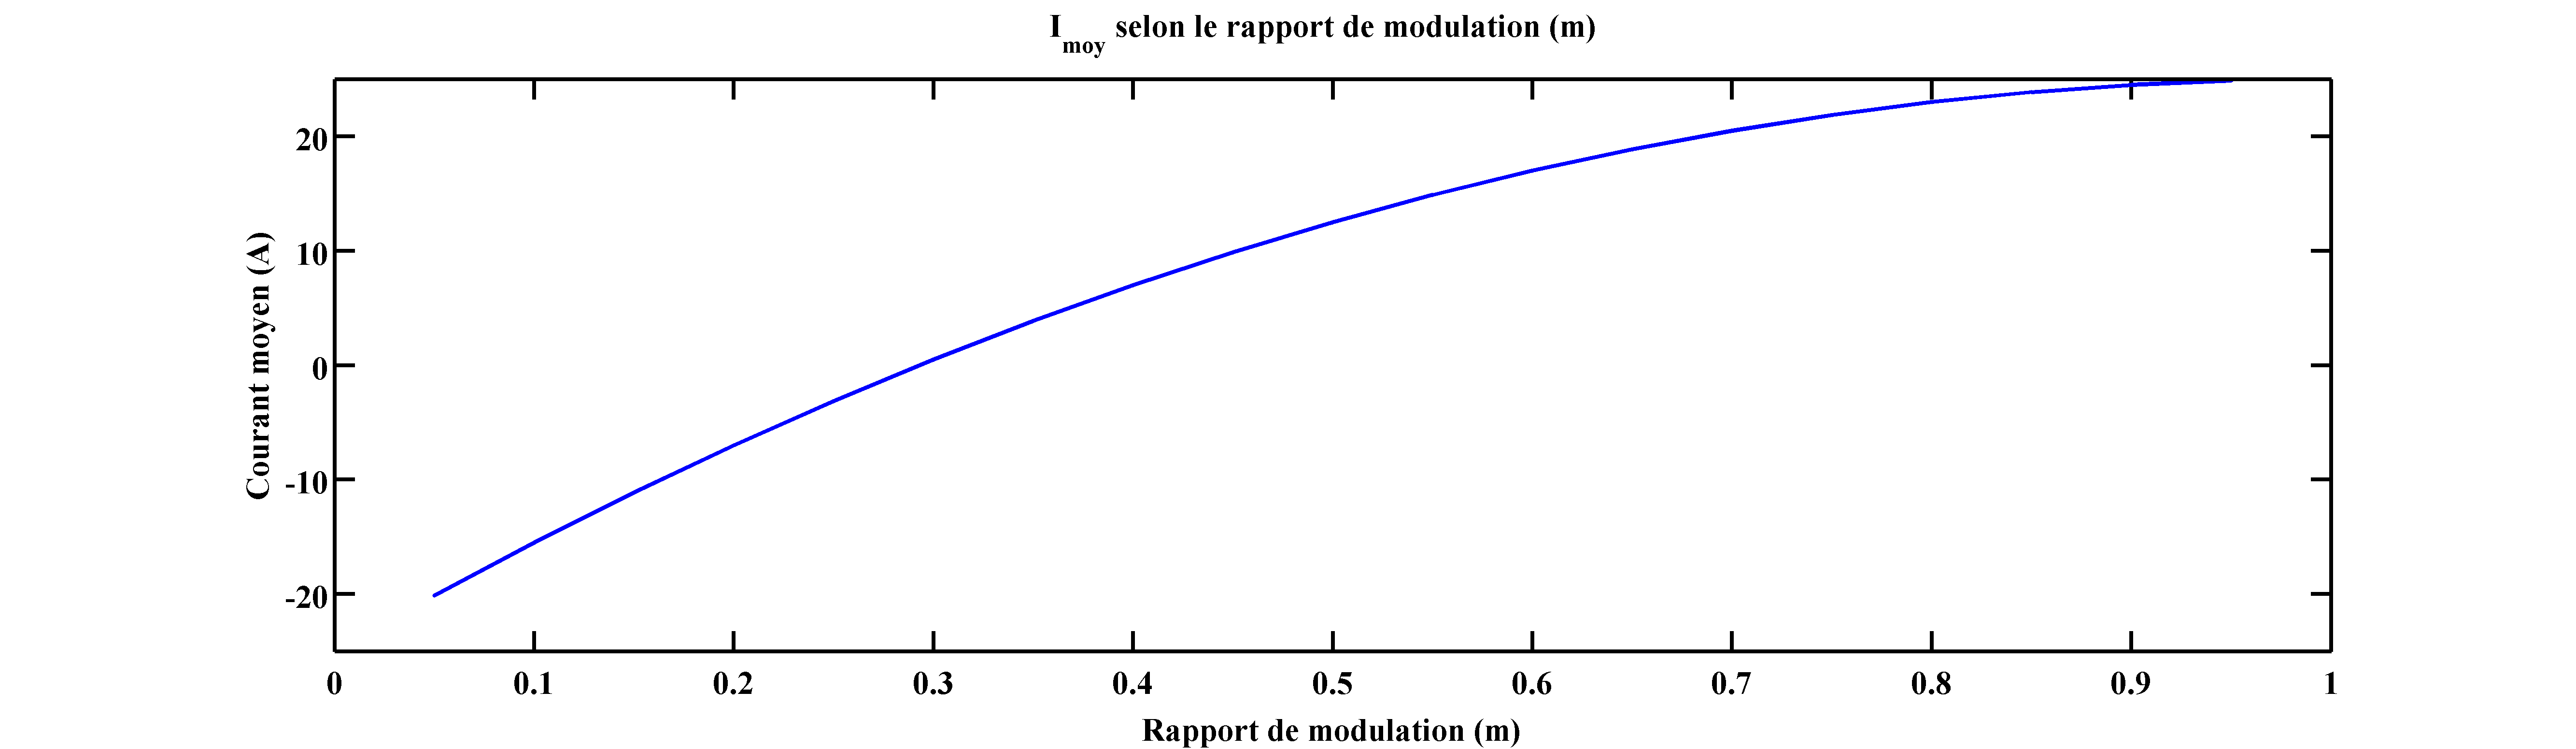
\includegraphics[scale=0.4]{Imoy_m.png}
\caption{Courant moyen en fonction du rapport de modulation dans un onduleur monophasé}
\end{figure}

\section{Fonctionnement d'un onduleur monophasé NPC à 3 niveaux}
Le schéma d'un onduleur monophasé NPC à 3 niveaux est présenté à la figure \ref{eq1}. Un onduleur monophasé NPC à 3 niveaux est composé de 4 transistors, de 6 diodes et de deux condensateurs rattachés au point neutre (point central sur la figure \ref{eq1}). La configuration présentée a pour objectif d'obtenir des niveaux distincts de tension $V_{DC}$ à appliquer aux bornes des électroaimants. Dans cette configuration, chaque transistor ne commute pas toute la tension $V_{DC}$, l'avantage étant qu'on peut utiliser des composantes dont le dimensionnement est moins imposant que celles nécessaire pour fournir une puissance équivalente dans un montage à 2 niveaux classique. 

\paragraph{}Il existe 4 transistors IGBT qui commutent par paires. Les séquences possibles et les tensions produites sont décrites dans le tableau suivant:

\begin{table}[htb]
\centering
\begin{tabular}{ |c|c|c| }
\hline
  Type de séquence & Transistors activés & Niveau de tension \\\hline\hline
  P & [1,2] & $+V_{DC}$ \\\hline
  N & [3,4] & $-V_{DC}$ \\\hline
  O & [1,3] & $0$ \\\hline
  O & [1,4] & $0$ \\\hline
  O & [2,4] & $0$ \\\hline
\end{tabular}
\end{table}

En excluant les états redondants, il existe 3 états distincts, soit l'état P ([1,2]), l'état N([3,4] et l'état 0([1,3]). Une stratégie de commande simple et applicable est celle d'une modulation MLI à plusieurs niveaux. On réfère ici à la figure \ref{fig_MLI_ML} pour une illustration graphique de la commande MLI multiniveaux. À chaque période de commutation, une comparaison entre l'onde désirée et le signal en dent de scie est effectuée. 

\begin{figure}[htb]
\centering
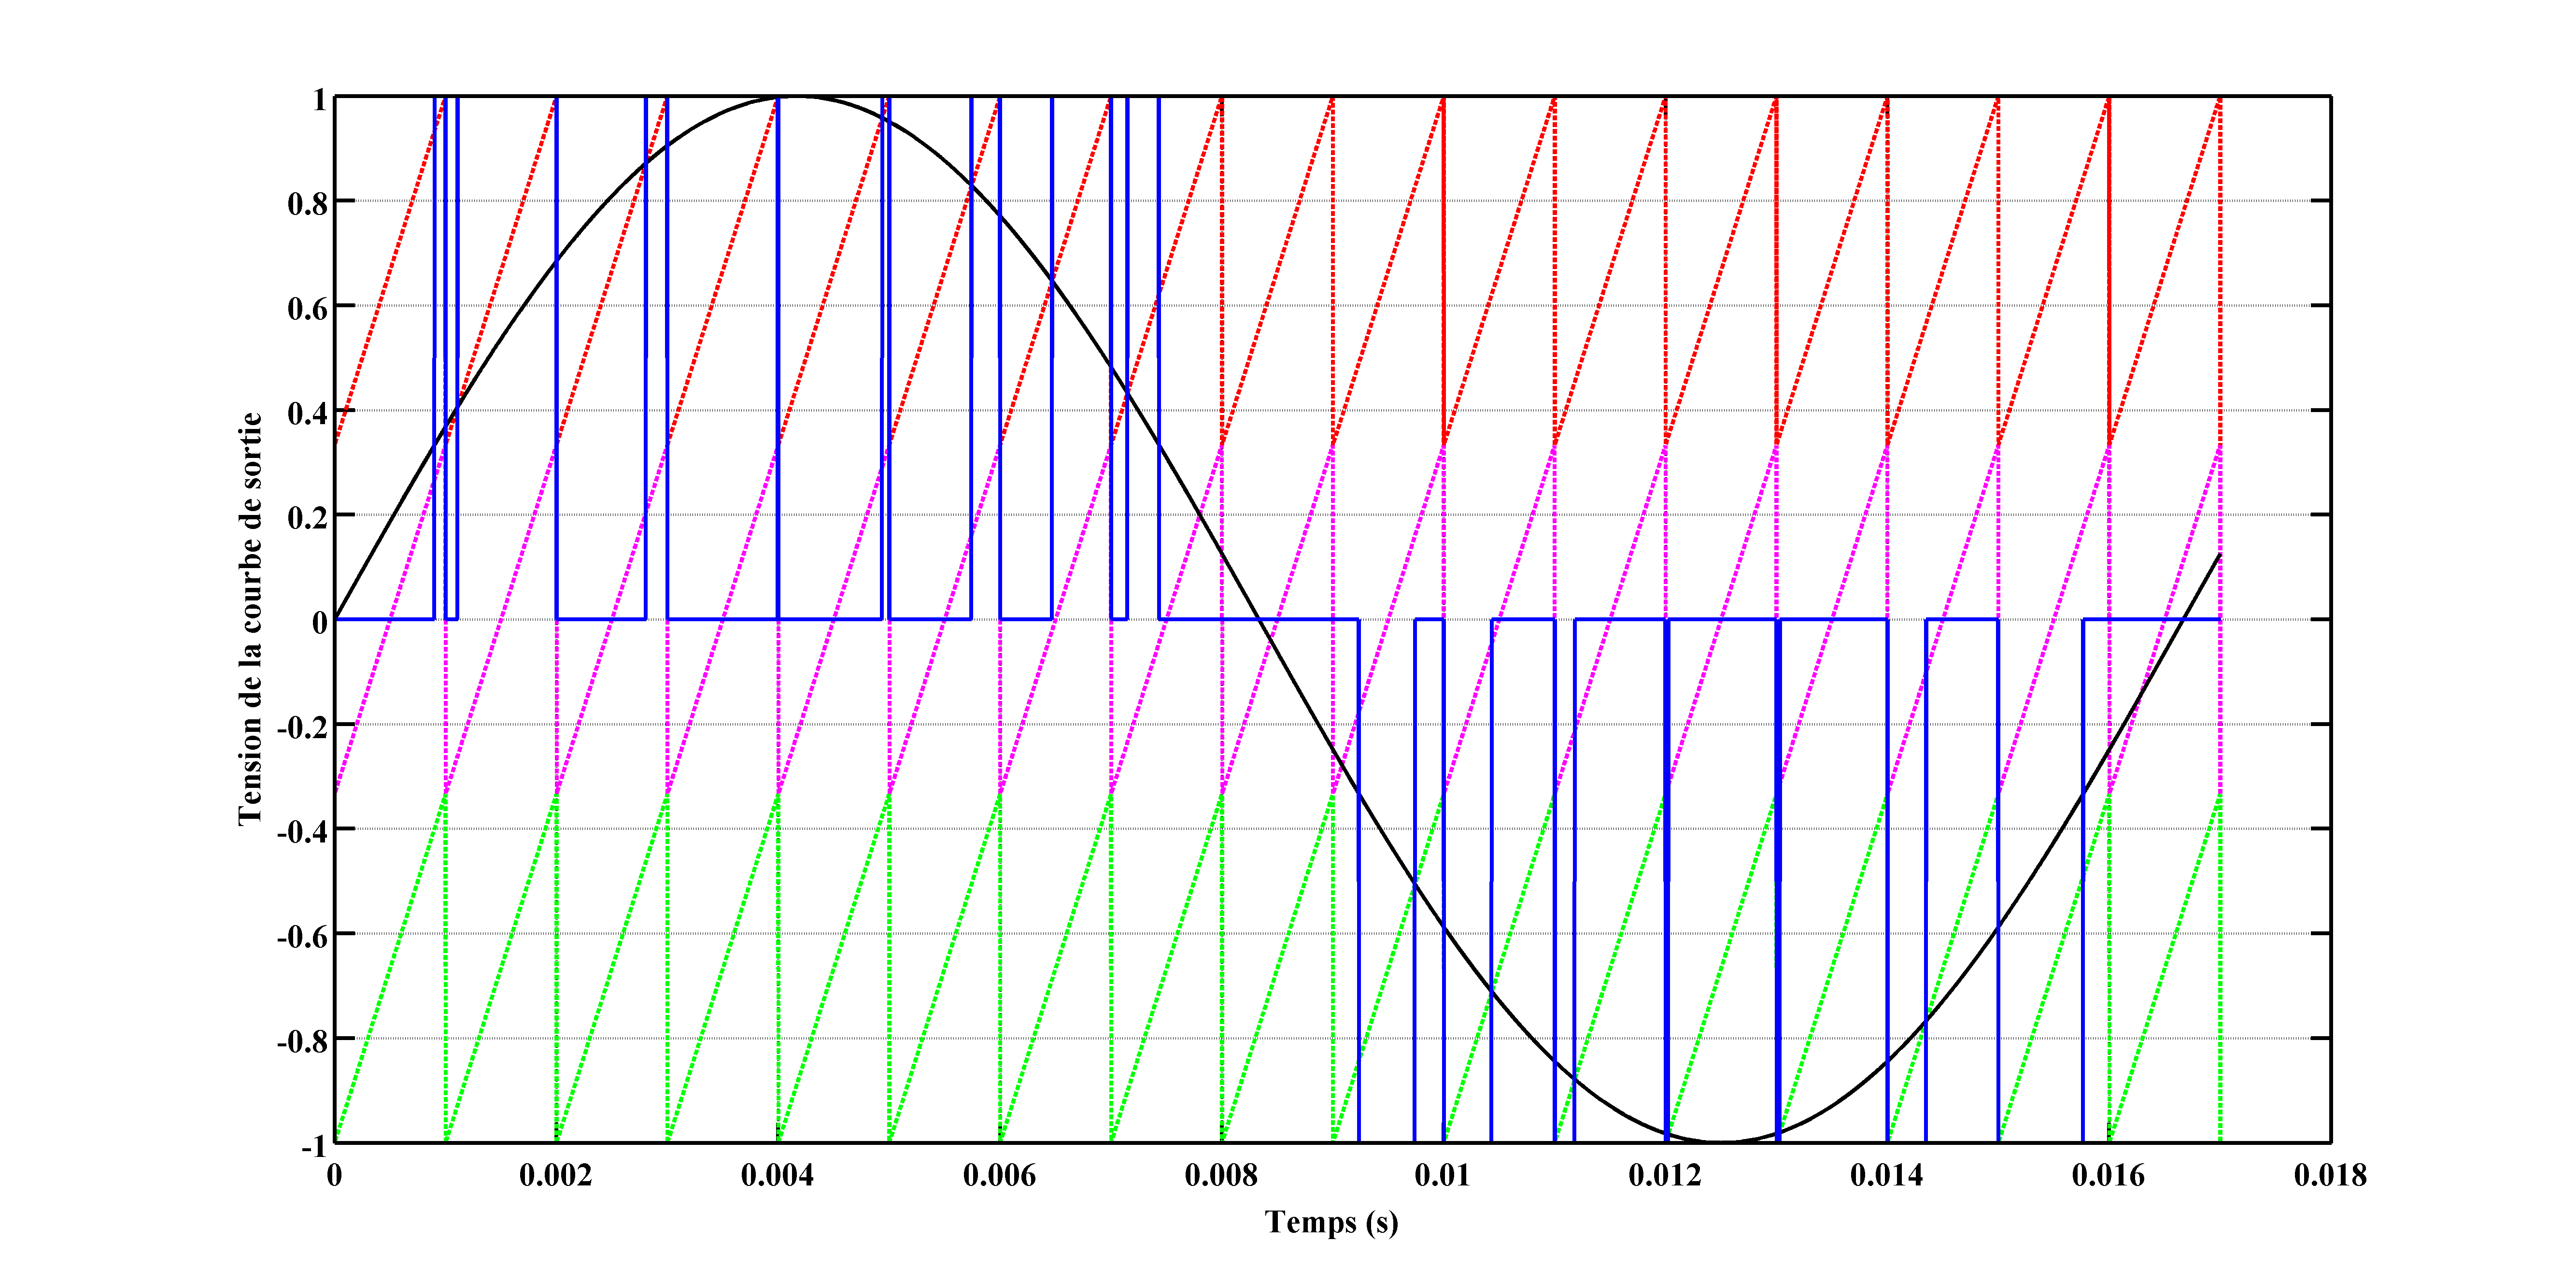
\includegraphics[scale=0.4]{commande_NPC_1.png}
\caption{Commande MLI multiniveaux pour une consigne sinusoïdale}
\label{fig_MLI_ML}
\end{figure}


\end{document}